\documentclass[11pt,a4paper,twoside]{book}
\usepackage[utf8]{inputenc}
\usepackage[spanish]{babel}
\usepackage{amsmath}
\usepackage{graphicx}
\usepackage{amsfonts}
\usepackage{amssymb}
\usepackage[left=2cm,right=2cm,top=2cm,bottom=2cm]{geometry}
\usepackage{float}
\author{Víctor de Tejada Molera}
\begin{document}
\chapter{Análisis estadístico}    
    
    En este apartado, se muestran los diferentes análisis que se han realizado para los diferentes test; así como los procedimientos utilizados para su obtención.
        
    \section{Análisis del test previo}
        Para este test sólo se pretende comprobar si las personas eran capaces de distinguir entre audios en posiciones muy diferentes. Por este motivo, se decidió realizar un análisis más sencillo que en el caso del test final. Más concretamente, se optó por utilizar la tabla A1 del anexo A de la norma UNE-EN ISO 10399\cite{ISO10399} (ver Anexo B del proyecto), así como la ecuación \ref{eq:alpha} ya mostrada en el capítulo de ``Estado del arte''.
            
        Aplicando dichos recursos se obtienen las tablas \ref{tablaResultadosDuda} y \ref{tablaResultadosSinDuda}: en la primera, se incluyen todas las respuestas y, en la segundam únicamente las que se marcaron como ``seguras'' por los participantes.
            
        \begin{table}[H]
	    \begin{center}
		\begin{scriptsize}
		\begin{tabular}{| c | c | c | c || c |}
			\hline
			\textbf{Separación butacas}&\textbf{Respuestas}&\textbf{Iguales}&\textbf{Diferentes}&\textbf{$\alpha$-risk}\\ \hline
            Horizontal&27&9&18&0.1\\ \hline
            Vertical&10&1&9&0.01\\ \hline
            Horizontal y vertical&23
            &5&18&0.01\\ \hline
            Misma posición&10&9&1&NO\\ \hline
		\end{tabular}
		\caption{Resultados del test previo.}
		\label{tablaResultadosDuda}
		\end{scriptsize}
		\end{center}	
		\end{table}	
		
		\begin{table}[H]
			\begin{center}
			\begin{scriptsize}
			\begin{tabular}{| c | c | c | c || c |}
			    \hline
				\textbf{Separación butacas}&\textbf{Respuestas}&\textbf{Iguales}&\textbf{Diferentes}&\textbf{$\alpha$-risk}\\ \hline
                Horizontal&23&7&16&0.05\\ \hline
                Vertical&9&1&8&0.05\\ \hline
                Horizontal y vertical&20&4&16&0.01\\ \hline
                Misma posición&9&8&1&NO\\ \hline
			\end{tabular}
			\caption{Resultados del test previo considerando las respuestas marcadas como ``Sin duda''.}
			\label{tablaResultadosSinDuda}
			\end{scriptsize}
			\end{center}	
		\end{table}
		
		Como se puede observar de las tablas, existen diferencias estadísticamente significativas cuando se separan los puntos de escucha. Esto se puede afirmar ya que se obtienen probabilidades bastante bajas de que las diferencias sean debidas al azar (entre 10\% y un 1\%). Dicho efecto se sigue manteniendo cuando se suprimen las respuestas marcadas como ``No seguras'', incluso se ve reforzado (el porcentaje de posibilidad de error se sitúa entre el 5\% y el1\%). Por este motivo, se considera probada nuestra primera hipótesis y se decidió continuar con el estudio. Para la situación de ``Misma posición'', se hano se alcanza el mínimo de respuestas correctas para alcanzar alguno de los valores de $\alpha$. Por este motivo, se representa en la tabla con un valor ``NO''. De esta forma, se marca que los participantes no han podido identificarlos como eventos distintos salvo por azar, lo cual era algo esperable puesto que se tratan de audios idénticos.
		
		Los valores concretos obtenidos para $\alpha$-risk no son realmente importantes, puesto que el número de datos es relativamente pequeño y la repetición de dicho experimentos podría producir que dichos valores fluctuaran. Para este caso, el experimento lo hemos considerado como válido al obtener valores inferiores o iguales a 0.1, que se corresponden a probabilidades de error menores o iguales al 10\%. (excepto para las respuestas en la misma posición).
		
    \section{Análisis del test final}
        Para el análisis del test final, se realizan dos análisis de datos diferentes para cada una de las dos formas de agrupación de los datos (distancia relativa a la fuente y distancia relativa entre las dos  butacas). El primer análisis se hará mediante el seguimiento de la norma UNE-EN ISO 10399 que ya se utilizó en el test previo, mediante la tabla A.1 de la norma y la ecuación \ref{eq:alpha}.
        
        Por otro lado, se realiza un análisis mediante modelos thurstonianos. Para ello, se genera un script en el lenguaje de programación estadística ``R'' para utilizar el paquete ``SensR''\footnote{https://cran.r-project.org/web/packages/sensR/index.html}. Este paquete permite obtener de forma sencilla los valores del coeficiente $d'$, así como su desviación estandar. En el anexo E puede consultarse el script.
        
        
		\subsection{Distancia relativa a la fuente}
		    Aplicando el mismo procedimiento explicado en apartado de ``Conceptos teóricos'', se obtienen los resultados para el análisis mediante la norma UNE-EN ISO 10399 para todas las respuestas y sólo para las marcadas como ``Nivel de seguridad: mucha'', respectivamente. También se utiliza el lenguaje de programación R y el paquete antes mencionado y así obtener el coeficiente $d'$ y su desviación estándar ($\sigma$). Todos los valores de ambos análisis están representados en las tablas \ref{tablaFuenteDuda} y \ref{tablaFuenteSinDuda}. Para la parte del análisis mediante modelos thurstonianos se generan además las figuras \ref{fig:ThurstFuenteDuda} y \ref{fig:ThurstFuenteSinDuda} que muestran de forma gráfica la variación de dicho coeficiente. El procedimiento para obtener el análisis con ``R'' es el siguiente: en primer lugar se introduce el núemero total de respuestas, así como el número de respuestas ``correctas'' (entendiéndose como correctas aquellas respuestas en las que los participantes hayan identificado los estímulos como diferentes). A continuación, hay que indicar a la función qué tipo de test se ha realizado para que el cálculo de los coeficientes sea el correcto. En nuestro caso, el test se corresponde con un ``\textit{2-AFC}'', ya que el participante estaba forzado a seleccionar una de las dos opciones sin posibilidad de escoger una opción intermedia.
		    
		    \begin{table}[H]
			\begin{center}
			\begin{scriptsize}
			\begin{tabular}{| c | c | c | c || c | c | c |}
			    \hline
				\textbf{Distancia [m]}&\textbf{Respuestas}&\textbf{Iguales}&\textbf{Diferentes}&\textbf{$\alpha$-Risk}&\textbf{$d'$}&\textbf{$\sigma (d')$}\\ \hline
                [6-8)&15&5&10&0.2&0.609&0.473\\ \hline
                [8-10)&35&10&25&0.05&0.800&0.318\\ \hline
                [10-11)&32&8&24&0.01&0.954&0.341\\ \hline
                [11-12)&53&12&41&0.001&1.062&0.270\\ \hline
                [12-13)&55&14&41&0.001&0.934&0.259\\ \hline
                [13-14)&67&14&53&0.001&1.146&0.244\\ \hline
                [14-15)&101&22&79&0.001&1.102&0.197\\ \hline
                [15-16)&99&18&81&0.001&1.285&0.208\\ \hline
                [16-17)&84&18&66&0.001&1.120&0.217\\ \hline
                [17-18)&63&10&53&0.001&1.414&0.269\\ \hline
                [18-19)&95&21&74&0.001&1.087&0.203\\ \hline
                [19-20)&62&19&43&0.01&0.715&0.236\\ \hline
                [20-21)&44&19&25&NO&0.243&0.269\\ \hline
                [21-24]&39&21&18&NO&0.000&NA\\ \hline
			\end{tabular}
			\caption{Valores de $\alpha$-risk, $d'$ y su desviación estandar para los resultados totales agrupados en función de la distancia a la fuente según la norma UNE-EN ISO 10399 y aplicando modelos thurstonianos, respectivamente.}
			\label{tablaFuenteDuda}
			\end{scriptsize}
			\end{center}	
		    \end{table}
		    
		    \begin{table}[H]
			\begin{center}
			\begin{scriptsize}
			\begin{tabular}{| c | c | c | c || c | c | c |}
			    \hline
				\textbf{Distancia [m]}&\textbf{Respuestas}&\textbf{Iguales}&\textbf{Diferentes}&\textbf{$\alpha$-risk}&\textbf{$d'$}&\textbf{$\sigma (d')$}\\ \hline
                [6-8)&11&3&8&0.2&0.855&0.571\\ \hline
                [8-10)&30&8&22&0.01&0.881&0.347\\ \hline
                [10-11)&23&6&17&0.05&0.906&0.399\\ \hline
                [11-12)&39&5&34&0.001&1.605&0.361\\ \hline
                [12-13)&47&11&36&0.001&1.026&0.285\\ \hline
                [13-14)&52&8&44&0.001&1.443&0.298\\ \hline
                [14-15)&81&12&69&0.001&1.477&0.241\\ \hline
                [15-16)&84&15&69&0.001&1.302&0.226\\ \hline
                [16-17)&68&12&56&0.001&1.314&0.252\\ \hline
                [17-18)&49&7&42&0.001&1.510&0.313\\ \hline
                [18-19)&77&18&59&0.001&1.027&0.223\\ \hline
                [19-20)&42&8&34&0.001&1.239&0.315\\ \hline
                [20-21)&25&10&15&No&0.358&0.359\\ \hline
                [21-24]&29&15&14&No&0&NA\\ \hline
			\end{tabular}
			\caption{Valores de $\alpha$-risk, $d'$ y su desviación estandar  para los resultados marcados como ``Sin duda'' agrupados en función de la distancia a la fuente según la norma UNE-EN ISO 10399 y aplicando modelos thurstonianos, respectivamente.}
			\label{tablaFuenteSinDuda}
			\end{scriptsize}
			\end{center}	
		    \end{table}
		    
		    
		    
		    \begin{figure}[H]
                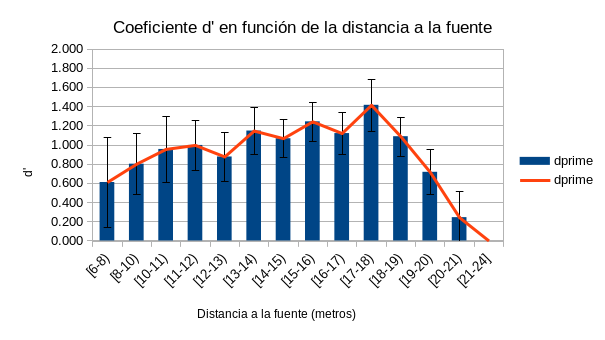
\includegraphics[scale=0.7]{../imagenes/analisisThurstFuenteDuda.png}
			    \centering
			    \caption{Coeficientes $d'$ y su desviación estándar en función de la distancia a la fuente.} 
			    \label{fig:ThurstFuenteDuda}
            \end{figure}
            
            \begin{figure}[H]
                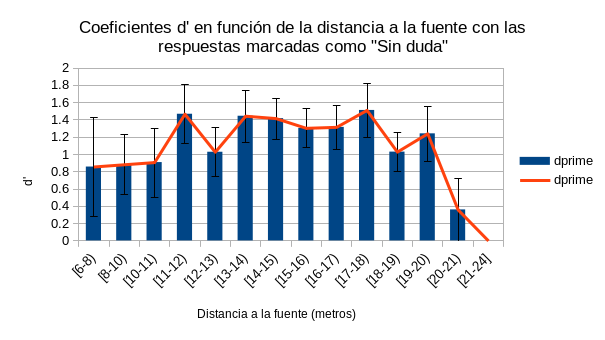
\includegraphics[scale=0.7]{../imagenes/analisisThurstFuenteSinDuda.png}
			    \centering
			    \caption{Coeficientes $d'$ y su desviación estándar en función de la distancia a la fuente cuando las respuestas están marcadas como ``Sin duda''.} 
			    \label{fig:ThurstFuenteSinDuda}
            \end{figure}

            Como se puede observar en las tablas y figuras antes mencionadas, el comportamiento para ambos procedimientos es bastante similar. Hay que tener en cuenta que para $\alpha$-risk, cuanto menor es el valor, estadísticamente más representativa es la diferencia, mientras que para los modelos thurstonianos, se produce a la inversa; cuanto mayor es el valor de $d'$, más diferentes son los estímulos.
            
            En ambos casos, se observa que las diferencias aumentan conforme aumenta la distancia respecto de la fuente, pero llegada una determinada distancia, las diferencias comienzan a dejar de ser perceptibles hasta llegar a posiciones donde las posibles diferencias pueden considerarse debidas al azar.
            
            La mayor diferencia entre ambos sistemas se encuentra en lo que podríamos denominar como ``sensibilidad''. La norma UNE-EN ISO 10399 es menos sensible a las variaciones puntuales del número de respuestas consideradas correctas; además de que los cambios que se producen son mucho más abruptos ya que sólo existen seis posibles valores para $\alpha$-risk (0.2, 0.1, 0.05, 0.01, 0.001 y que no pueda obtenerse el valor).
            
            Los modelos thurstonianos, por otra parte, son mucho más sensibles, ya que ligeras variaciones en los resultados, producen variaciones en los valores de $d'$. Al mismo tiempo, se dispone de todo un rango contínuo de valores que dicho coeficiente puede obtener. Esto permite que las representaciones gráficas de las variaciones de $d'$ muestren mejor el comportamiento psicoacústico de los estímulos y analizar si existe una tendencia, como es el caso de nuestro experimento.
            
            Un ejemplo de esto puede observarse en los casos de la tabla \ref{tablaFuenteDuda}. En esta tabla, se ve como para el caso del análisis mediante la norma, el descenso se produce a partir de la distancia de [19-20) metros, mientras que en los modelos thurstonianos, el decaimiento se produce antes, a partir de la distancia [18-19) metros. Lo mismo ocurre con el caso de la tabla \ref{tablaFuenteSinDuda}, donde los decaimientos vuelven a producirse en las mismas distancias. Para tener una idea de este comportamiento sobre el espacio del auditorio, se presenta la figura \ref{fig:dprimeauditorio}, donde se representa el comportamiento de $d'$ (la percepción de diferencia entre parejas de estímulos) en función de dicha distancia en la fuente, pero representado sobre el plano del auditorio directamente mediante un diagrama de colores en el que las zonas verdes representan valores bajos de dichas diferencias perceptuales y las zonas rojas representan valores elevados. Las zonas sin pintar corresponden a zonas donde o bien no se han tomado medidas, o bien el valor de las diferencias perceptuales ($d'$) es nulo. También se ha considerado que el comportamiento de la sala es simétrico respecto al eje longitudinal de la sala y que, para la zona delantera donde no hay butacas, se ha realizado una extrapolación de los datos.
            
            \begin{figure}[H]
                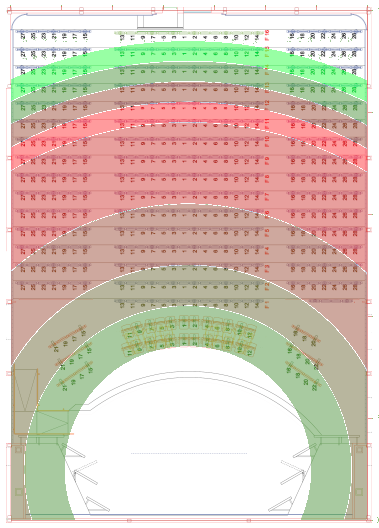
\includegraphics[scale=0.9]{../imagenes/auditoriodprime.png}
			    \centering
			    \caption{Coeficientes $d'$ en función de la distancia a la fuente representado sobre el plano del auditorio. Los valores verdes representan un valor bajo de $d'$; mientras que los rojos representan valores elevados.} 
			    \label{fig:dprimeauditorio}
            \end{figure}
        
        \subsection{Distancia relativa entre butacas}
            Para este apartado se vuelven a aplicar tanto los procedimientos de la norma UNE-EN ISO 10399, como los modelos thusthonianos. De ambos análisis se obtienen las tablas \ref{tablaButacasDuda} y \ref{tablaButacasSinDuda}, así como las figuras \ref{fig:ThurstButacasDuda} y \ref{fig:ThurstButacasSinDuda}. De nuevo, para los modelos thurstonianos, se ha determinado que el protocolo es ``\textit{2-AFC}'' para que la función de R pueda realizar de forma correcta la estimación del valor $d'$.
            
            Como se puede observar en las tablas recien mencionadas, los participantes empiezan a notar diferencias cuando la distancia entre butacas se encuentra a partir de los [3-4) metros, aunque este efecto se retrasa hasta los [4-5) metros si suprimimos las respuestas marcadas como ``Con duda''. Una vez ahí, las diferencias se mantienen estadísticamente representativas con el máximo nivel de seguridad que ofrece la norma, ya que la probabilidad de que los eventos sean iguales cuando, en realidad, se han percibido como diferentes, es de 0.001. En los resultados obtenidos no hay un momento en el que dicha probabilidad decrezca.
            
            \begin{table}[H]
			\begin{center}
			\begin{scriptsize}
			\begin{tabular}{| c | c | c | c || c | c | c |}
			    \hline
				\textbf{Distancia [m]}&\textbf{Respuestas}&\textbf{Total iguales}&\textbf{Total diferentes}&\textbf{$\alpha$-risk}&\textbf{$d'$}&\textbf{$\sigma (d')$}\\ \hline
                (0-2)&61&40&21&NO&0.000&NA\\ \hline
                [2-3)&76&40&36&NO&0.000&NA\\ \hline
                [3-4)&102&47&55&0.05&0.139&0.176\\ \hline
                [4-5)&111&30&81&0.001&0.865&0.18\\ \hline0
                [5-6)&95&24&71&0.001&0.942&0.197\\ \hline
                [6-7)&78&11&67&0.001&1.521&0.249\\ \hline
                [7-8)&70&9&61&0.001&1.603&0.270\\ \hline
                [8-9)&52&4&48&0.001&2.017&0.362\\ \hline
                [9-10)&62&3&59&0.001&2.349&0.384\\ \hline
                [10-11)&47&1&46&0.001&2.868&0.583\\ \hline
                [11-12)&33&1&32&0.001&2.654&0.615\\ \hline
                [12-14)&33&1&32&0.001&2.654&0.615\\ \hline
                [14-18)&24&0&24&0.001&$\infty$&NA\\ \hline
			\end{tabular}
			\caption{Valores de $\alpha$-risk, $d'$ y su desviación estándar para los resultados totales agrupados en función de la distancia entre butacas según la norma UNE-EN ISO 10399 y aplicando modelos thurstonianos, respectivamente.}
			\label{tablaButacasDuda}
			\end{scriptsize}
			\end{center}	
		    \end{table}
		    
		    \begin{table}[H]
			\begin{center}
			\begin{scriptsize}
			\begin{tabular}{| c | c | c | c || c | c | c |}
			    \hline
				\textbf{Distancia [m]}&\textbf{Respuestas}&\textbf{Total iguales}&\textbf{Total diferentes}&\textbf{$\alpha$-risk}&\textbf{$d'$}&\textbf{$\sigma (d')$}\\ \hline
                (0-2)&41&27&14&NO&0.000&NA\\ \hline
                [2-3)&49&29&20&NO&0.000&NA\\ \hline
                [3-4)&74&33&41&NO&0.192&0.207\\ \hline
                [4-5)&79&17&62&0.001&1.115&0.224\\ \hline
                [5-6)&65&15&50&0.001&1.041&0.243\\ \hline
                [6-7)&62&5&57&0.001&1.981&0.327\\ \hline
                [7-8)&64&7&57&0.001&1.739&0.295\\ \hline
                [8-9)&40&1&39&0.001&2.772&0.597\\ \hline
                [9-10)&53&2&51&0.001&2.514&0.450\\ \hline
                [10-11)&44&1&43&0.001&2.829&0.589\\ \hline
                [11-12)&31&1&30&0.001&2.614&0.621\\ \hline
                [12-14)&32&0&32&0.001&$\infty$&NA\\ \hline
                [14-18)&23&0&23&0.001&$\infty$&NA\\ \hline
			\end{tabular}
			\caption{Valores de $\alpha$-risk, $d'$ y se desviación estándar para los resultados agrupados en función de la distancia entre butacas según la norma UNE-EN ISO 10399 y aplicando modelos thurstonianos, respectivamente, cuando los resultados son marcados como ``Sin duda''.}
			\label{tablaButacasSinDuda}
			\end{scriptsize}
			\end{center}	
		    \end{table}
            
            
            Por otro lado, la tabla \ref{tablaButacasDuda}, así como la figura \ref{fig:ThurstButacasDuda}, muestran, para el análisis mediante modelos thurstonianos, un crecimiento más o menos constante del coeficiente $d'$ desde los [3-4) metros hasta el final. En este caso, en el que están incluidos los resultados marcados como ``Con duda'', puede parecer que existe una bajada de la percepción de las diferencias, pero al observar los datos de la tabla, se ve que ese decaimiento se debe a que se tienen menos datos en dichas posiciones y, por tanto, el hecho de que una persona determine que ha percibido los audios como iguales, hace que el valor del coeficiente baje. Esto se comprueba observando la tabla \ref{tablaButacasSinDuda} y figura \ref{fig:ThurstButacasSinDuda} donde se han eliminado las respuestas dudosas y se observa un reforzamiento en la tendencia creciente en las distancias más lejanas.
		    
		    \begin{figure}
                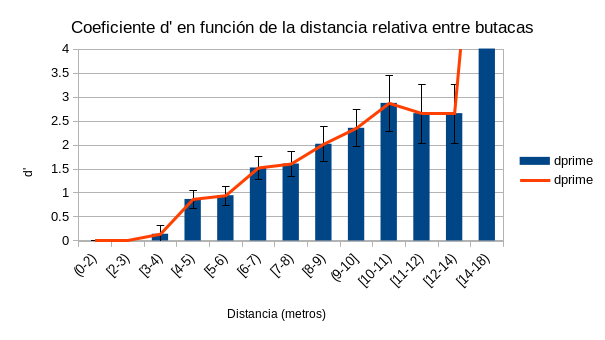
\includegraphics[scale=0.7]{../imagenes/analisisThurstButacasDuda.png}
			    \centering
			    \caption{Coeficientes $d'$ y su desviación estándar en función de la distancia entre butacas.} 
			    \label{fig:ThurstButacasDuda}
            \end{figure}
            
            \begin{figure}
                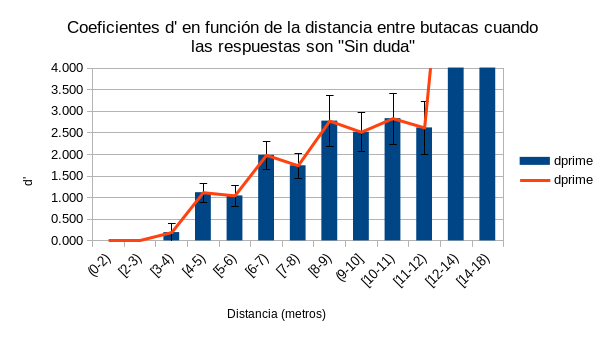
\includegraphics[scale=0.7]{../imagenes/analisisThurstButacasSinDuda.png}
			    \centering
			    \caption{Coeficientes $d'$ y su desviación estándar en función de la distancia entre butacas cuando las respuestas están marcadas como ``Sin duda''.} 
			    \label{fig:ThurstButacasSinDuda}
            \end{figure}
            
            Al igual que ocurría con los resultados agrupados según la distancia a la fuente, se observa que, a pesar, de que el comportamiento es similar para ambas formas de analizar los datos, la norma UNE-EN ISO 10399\cite{ISO10399} es mucho menos sensible a los pequeños cambios en los resultados; mientras que los modelos thurstonianos ofrecen un rango mayor de datos que fluctúan más facilmente. Esto no es necesariamente peor; depende de lo que se pretenda conseguir con el estudio. Si se pretende determinar a partir de qué distancias las diferencias son significativas, la norma da información más útil en este sentido. Por otro lado, si se pretende estudiar el comportamiento de las diferencias perceptuales en función de la distancia, aquí los modelos thurstonianos tienen una gran ventaja frente a la norma.
		    
		    
   
\end{document}